\documentclass{report}
\usepackage{graphicx, tikz-cd, float, titlepic, booktabs} % Required for inserting images
\usepackage{pgfplots}
\pgfplotsset{compat=1.15}
\usepackage{mathrsfs}
\usetikzlibrary{arrows}
\usepackage{amsmath, amssymb, amsthm, amsfonts, siunitx, physics, gensymb}
\AtBeginDocument{\RenewCommandCopy\qty\SI}
\usepackage[version=4]{mhchem}
\usepackage[most,many,breakable]{tcolorbox}
\usepackage{xcolor, fancyhdr, varwidth}
\usepackage[Glenn]{fncychap}
%Options: Sonny, Lenny, Glenn, Conny, Rejne, Bjarne, Bjornstrup
\usepackage{hyperref, cleveref}
\usepackage{icomma, enumitem} %comma as decimal and continue enumerate with [resume]
\usepackage{plimsoll} %use standard state symbol with \stst
\usepackage[danish]{babel}
%%%%%%%%%%%%%%%%%%%%%%%%%%%%%%
% SELF MADE COLORS
%%%%%%%%%%%%%%%%%%%%%%%%%%%%%%
\definecolor{myg}{RGB}{56, 140, 70}
\definecolor{myb}{RGB}{45, 111, 177}
\definecolor{myr}{RGB}{199, 68, 64}
\definecolor{mytheorembg}{HTML}{F2F2F9}
\definecolor{mytheoremfr}{HTML}{00007B}
\definecolor{mylenmabg}{HTML}{FFFAF8}
\definecolor{mylenmafr}{HTML}{983b0f}
\definecolor{mypropbg}{HTML}{f2fbfc}
\definecolor{mypropfr}{HTML}{191971}
\definecolor{myexamplebg}{HTML}{F2FBF8}
\definecolor{myexamplefr}{HTML}{88D6D1}
\definecolor{myexampleti}{HTML}{2A7F7F}
\definecolor{mydefinitbg}{HTML}{E5E5FF}
\definecolor{mydefinitfr}{HTML}{3F3FA3}
\definecolor{notesgreen}{RGB}{0,162,0}
\definecolor{myp}{RGB}{197, 92, 212}
\definecolor{mygr}{HTML}{2C3338}
\definecolor{myred}{RGB}{127,0,0}
\definecolor{myyellow}{RGB}{169,121,69}
\definecolor{myexercisebg}{HTML}{F2FBF8}
\definecolor{myexercisefg}{HTML}{88D6D1}
%%%%%%%%%%%%%%%%%%%%%%%%%%%%%%%%%%%%%%%%%%%%%%%%%%%%%%%%%%%%%%%%%%%%%%
% Box environments for theorems and problems
%%%%%%%%%%%%%%%%%%%%%%%%%%%%%%%%%%%%%%%%%%%%%%%%%%%%%%%%%%%%%%%%%%%%%
\setlength{\parindent}{1cm}
%================================
% Question BOX
%================================
\makeatletter
\newtcbtheorem{question}{Opgave}{enhanced,
	breakable,
	colback=white,
	colframe=myb!80!black,
	attach boxed title to top left={yshift*=-\tcboxedtitleheight},
	fonttitle=\bfseries,
	title={#2},
	boxed title size=title,
	boxed title style={%
			sharp corners,
			rounded corners=northwest,
			colback=tcbcolframe,
			boxrule=0pt,
		},
	underlay boxed title={%
			\path[fill=tcbcolframe] (title.south west)--(title.south east)
			to[out=0, in=180] ([xshift=5mm]title.east)--
			(title.center-|frame.east)
			[rounded corners=\kvtcb@arc] |-
			(frame.north) -| cycle;
		},
	#1
}{def}
\makeatother
%================================
% DEFINITION BOX
%================================

\newtcbtheorem[]{Definition}{Definition}{enhanced,
	before skip=2mm,after skip=2mm, colback=red!5,colframe=red!80!black,boxrule=0.5mm,
	attach boxed title to top left={xshift=1cm,yshift*=1mm-\tcboxedtitleheight}, varwidth boxed title*=-3cm,
	boxed title style={frame code={
					\path[fill=tcbcolback]
					([yshift=-1mm,xshift=-1mm]frame.north west)
					arc[start angle=0,end angle=180,radius=1mm]
					([yshift=-1mm,xshift=1mm]frame.north east)
					arc[start angle=180,end angle=0,radius=1mm];
					\path[left color=tcbcolback!60!black,right color=tcbcolback!60!black,
						middle color=tcbcolback!80!black]
					([xshift=-2mm]frame.north west) -- ([xshift=2mm]frame.north east)
					[rounded corners=1mm]-- ([xshift=1mm,yshift=-1mm]frame.north east)
					-- (frame.south east) -- (frame.south west)
					-- ([xshift=-1mm,yshift=-1mm]frame.north west)
					[sharp corners]-- cycle;
				},interior engine=empty,
		},
	fonttitle=\bfseries,
	title={#2},#1}{def}
\newtcbtheorem[]{definition}{Definition}{enhanced,
	before skip=2mm,after skip=2mm, colback=red!5,colframe=red!80!black,boxrule=0.5mm,
	attach boxed title to top left={xshift=1cm,yshift*=1mm-\tcboxedtitleheight}, varwidth boxed title*=-3cm,
	boxed title style={frame code={
					\path[fill=tcbcolback]
					([yshift=-1mm,xshift=-1mm]frame.north west)
					arc[start angle=0,end angle=180,radius=1mm]
					([yshift=-1mm,xshift=1mm]frame.north east)
					arc[start angle=180,end angle=0,radius=1mm];
					\path[left color=tcbcolback!60!black,right color=tcbcolback!60!black,
						middle color=tcbcolback!80!black]
					([xshift=-2mm]frame.north west) -- ([xshift=2mm]frame.north east)
					[rounded corners=1mm]-- ([xshift=1mm,yshift=-1mm]frame.north east)
					-- (frame.south east) -- (frame.south west)
					-- ([xshift=-1mm,yshift=-1mm]frame.north west)
					[sharp corners]-- cycle;
				},interior engine=empty,
		},
	fonttitle=\bfseries,
	title={#2},#1}{def}

\newtcbtheorem{theo}%
    {Theorem}{}{theorem}
\newtcolorbox{prob}[1]{colback=red!5!white,colframe=red!50!black,fonttitle=\bfseries,title={#1}}
%================================
% NOTE BOX
%================================

\usetikzlibrary{arrows,calc,shadows.blur}
\tcbuselibrary{skins}
\newtcolorbox{note}[1][]{%
	enhanced jigsaw,
	colback=gray!20!white,%
	colframe=gray!80!black,
	size=small,
	boxrule=1pt,
	title=\textbf{Note:},
	halign title=flush center,
	coltitle=black,
	breakable,
	drop shadow=black!50!white,
	attach boxed title to top left={xshift=1cm,yshift=-\tcboxedtitleheight/2,yshifttext=-\tcboxedtitleheight/2},
	minipage boxed title=1.5cm,
	boxed title style={%
			colback=white,
			size=fbox,
			boxrule=1pt,
			boxsep=2pt,
			underlay={%
					\coordinate (dotA) at ($(interior.west) + (-0.5pt,0)$);
					\coordinate (dotB) at ($(interior.east) + (0.5pt,0)$);
					\begin{scope}
						\clip (interior.north west) rectangle ([xshift=3ex]interior.east);
						\filldraw [white, blur shadow={shadow opacity=60, shadow yshift=-.75ex}, rounded corners=2pt] (interior.north west) rectangle (interior.south east);
					\end{scope}
					\begin{scope}[gray!80!black]
						\fill (dotA) circle (2pt);
						\fill (dotB) circle (2pt);
					\end{scope}
				},
		},
	#1,
}
%================================
% EXAMPLE BOX
%================================
\newtcbtheorem[number within=section]{Example}{Example}
{%
	colback = myexamplebg
	,breakable
	,colframe = myexamplefr
	,coltitle = myexampleti
	,boxrule = 1pt
	,sharp corners
	,detach title
	,before upper=\tcbtitle\par\smallskip
	,fonttitle = \bfseries
	,description font = \mdseries
	,separator sign none
	,description delimiters parenthesis
}
{ex}
%================================
% THEOREM BOX
%================================

\tcbuselibrary{theorems,skins,hooks}
\newtcbtheorem[number within=section]{Theorem}{Theorem}
{%
	enhanced,
	breakable,
	colback = mytheorembg,
	frame hidden,
	boxrule = 0sp,
	borderline west = {2pt}{0pt}{mytheoremfr},
	sharp corners,
	detach title,
	before upper = \tcbtitle\par\smallskip,
	coltitle = mytheoremfr,
	fonttitle = \bfseries\sffamily,
	description font = \mdseries,
	separator sign none,
	segmentation style={solid, mytheoremfr},
}
{th}

%%%%%%%%%%%%%%%%%%%%%%%%%%%%%%%%%%%%%%%%%%%%%%%%%%%%%%%%%%%%%%%%%
% SELF MADE COMMANDS
%%%%%%%%%%%%%%%%%%%%%%%%%%%%%%
\newcommand{\sol}{\setlength{\parindent}{0cm}\textbf{\textit{Løsning:}}\setlength{\parindent}{1cm}}
%%%%%%%%%%%%%%%%%%%%%%%%%%%%%%%%%
\usepackage[tmargin=2cm,rmargin=1in,lmargin=1in,margin=0.85in,bmargin=2cm,footskip=.2in]{geometry}\pagestyle{fancy}
\lhead{Minrui Kevin Zhou 3.b}
\rhead{H6}

\title{H6\\
{\Large \textbf{3.b fysik A}}}
\author{Kevin Zhou}
\date{\today}

\begin{document}
\maketitle
\begin{question}{Fodbold}{}
  En fodbold har farten 31,1 m/s. Fodboldens formfaktor er 0,26, og dens tværsnitsareal er $0,038 \;\unit{m^2} $. 
  \begin{itemize}
    \item[a.] Beregn størrelsen af luftmodstanden på fodbolden.
  \end{itemize}
Bilaget Fodbold er en video, som viser en fod, der sparker til en fodbold. Videoen er optaget med 10000 billeder pr. sekund. Fodbolden har massen 0,435 kg, og dens diameter er 0,22 m.
\begin{itemize}
  \item[b.] Benyt videoen til at vurdere storrelsen af den gennemsnitlige samlede kraft pa fodbolden under sparket.
\end{itemize}
\end{question}
\sol \\
\textbf{a.}
Da fodbolden bevæger sig relativt hurtigt, må der være tale om turbulent strømning.
Ved $20 \;\unit{\celsius} $ og et tryk på $1 \;\unit{atm} $ er luftens densitet $1,205 \;\unit{kg/m^3} $. 
Vi kan da beregne størrelsen af luftmodstanden med $v^2$-loven.
\begin{equation*}
\begin{split}
  |\va{F} _{\text{luft} }| &= \frac{1}{2} \cdot c_w \cdot \rho \cdot A \cdot v^2\\
  &=\frac{1}{2} \cdot 0,26 \cdot 1,205 \;\unit{kg/m^3} \cdot 0,038 \;\unit{m^2} \cdot \left(31,1 \;\unit{m/s} \right)^2\\
  &\approx 5,8 \;\unit{N}
\end{split}
\end{equation*}
Altså er størrelsen af luftmodstanden på bolden $5,8 \;\unit{N} $. \\[1ex]
\textbf{b.}
En videoanalyse laves i Logger Pro, hvilket ses i \cref{fig:video}.
Boldens diameter bruges som målestok.
\begin{figure}[H]
\begin{center}
  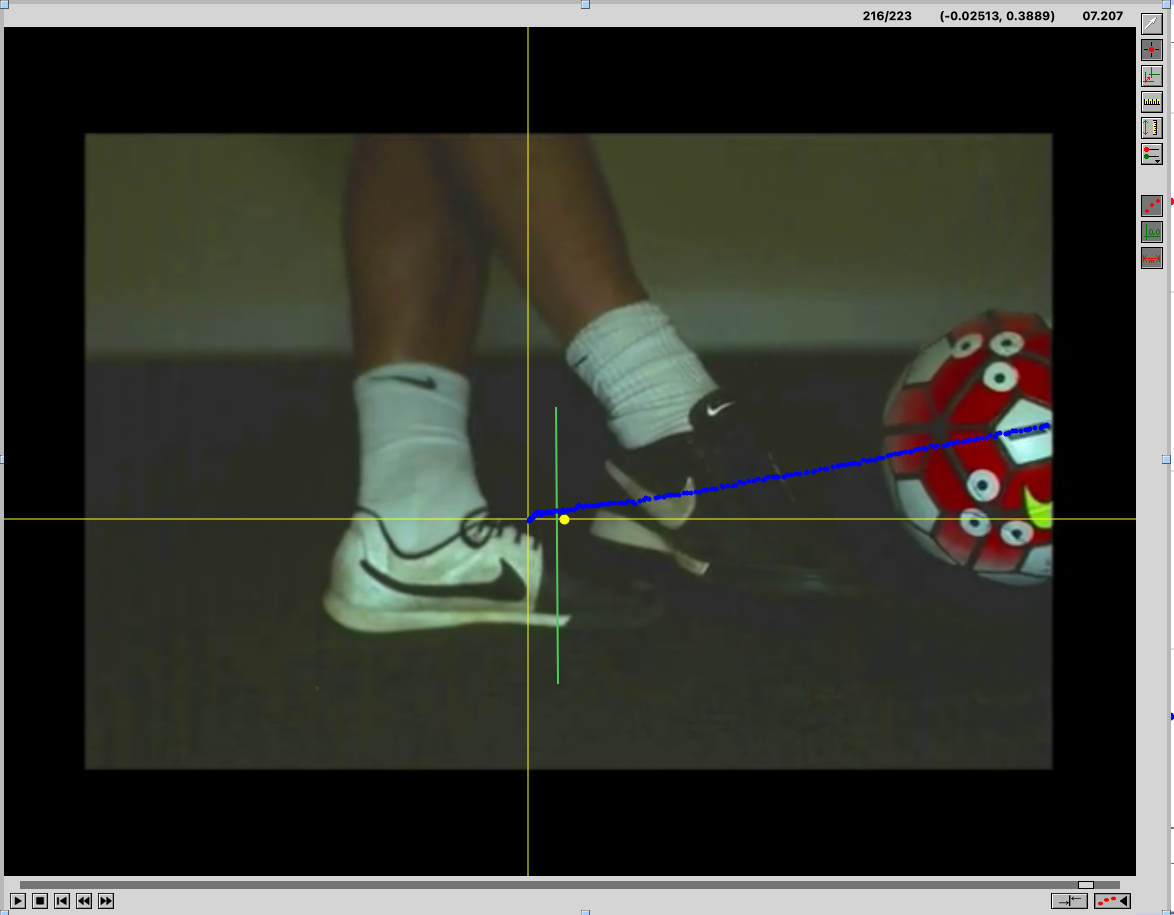
\includegraphics[width=0.7\textwidth]{video-analyse.png}
\end{center}
\caption{Videoanalyse af bevægelsen}
\label{fig:video}
\end{figure}
En ny beregnet kolonne laves med afstand fra startpunktet, hvor 
\[
\text{Afstand} = \sqrt{x^2+y^2} 
\] 
Hældningen på $(t,\text{Afstand} )$-grafen må være boldens fart.
Når vi ser bort fra luftmodstand, må boldens fart være konstant efter den har forladt foden (hvilket passer tilnærmelsesvist, da vi undersøger et meget kort tidsinterval).
Denne betegner vi for $v_{\text{efter} }$ og bestemmes via lineær regression på den sidste del af bevægelsen (hvor bolden har forladt foden), hvilket ses i \cref{fig:v}.
\begin{figure}[H]
\begin{center}
  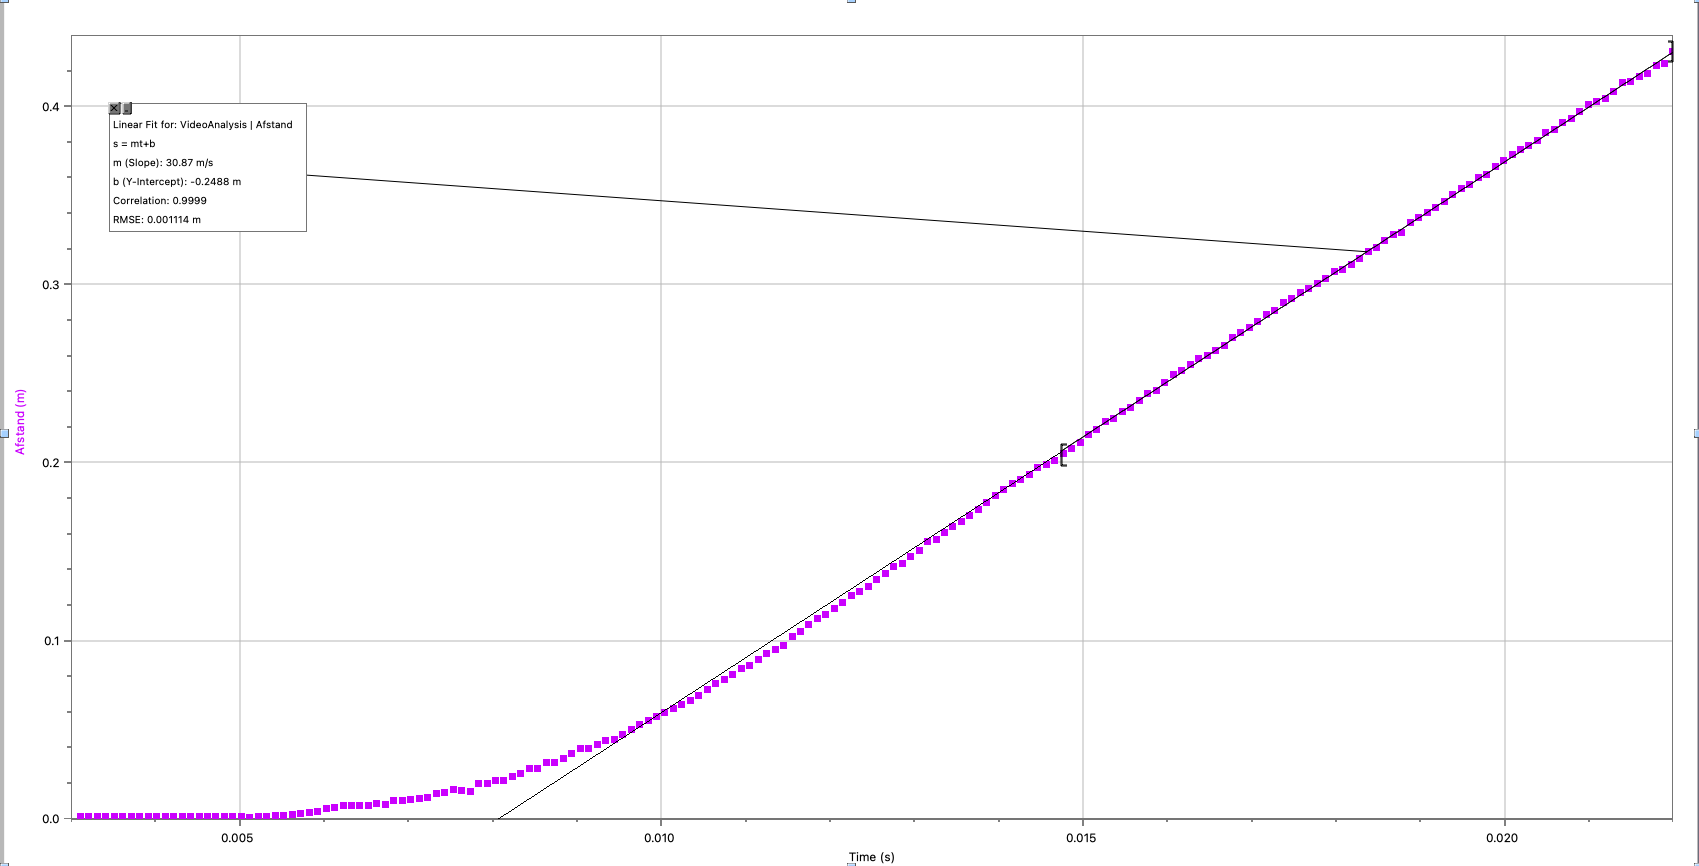
\includegraphics[width=\textwidth]{v.png}
\end{center}
  \caption{Lineær regression på $(t, \text{Afstand}  )$-grafen i Logger Pro}
\label{fig:v}
\end{figure}
Fra regressionen har vi 
\[
v _{\text{efter} }=30,87 \;\unit{m/s} 
\] 
På videoen ses det, at sparket varer $0,014 \;\unit{s} $.
Da bolden starter fra hvile, gælder der ifølge impulssætningen for størrelsen af den gennemsnitlige samlede kraft på bolden (bemærk at vi herunder blot beregner størrelsen af den \textit{gennemsnitlige} samlede kraft, da $F$ ikke nødvendigvis er konstant og kan være varierende), at 
\begin{equation*}
\begin{split}
  F&=\frac{\Delta p}{\Delta t}\\
  &=\frac{m \cdot v_{\text{efter} } - 0 \;\unit{\frac{kg \cdot m}{s}} }{\Delta t }\\
  &=\frac{0,435 \;\unit{kg} \cdot 30,87 \;\unit{m/s} }{0,014 \;\unit{s} }\\
  &\approx 9,6 \cdot 10^2 \;\unit{N} \\
  &=0,96 \;\unit{kN} 
\end{split}
\end{equation*}
Størrelsen af den gennemsnitlige samlede kraft på fodbolden under sparket er altså $0,96 \;\unit{kN} $.

\begin{question}{Stempelkande}{}
  Når stemplet i en stempelkande presses ned, er stemplet påvirket af flere kræfter herunder en kraft, der skyldes opdriften på kaffegrumset. Kaffegrumset har rumfanget $235 \;\unit{cm^3} $.
  \begin{itemize}
    \item[a.] Hvor stor er opdriften på kaffegrumset?
  \end{itemize}
Stemplet bliver presset ned. Grafen viser sammenhørende værdier for stemplets position $s$ og størrelsen af håndens kraft $F$ på stemplet.
\begin{itemize}
  \item[b.] Vurder håndens arbejde på stemplet, når det trykkes ned.
\end{itemize}
\end{question}
\sol \\
\textbf{a.}
Vi antager, at kaffen har samme densitet som vand.
Fra Archimedes' lov om opdrift har vi
\begin{equation*}
\begin{split}
  F _{\text{op} }&= \rho \cdot V \cdot g \\
  &=1000 \;\unit{kg/m^3} \cdot 235 \cdot 10 ^{-6} \;\unit{m^3} \cdot 9,82 \;\unit{m/s^2} \\
  &\approx 2,31 \;\unit{N} 
\end{split}
\end{equation*}
Altså er størrelsen på opdriften på kaffegrumset $2,31 \;\unit{N} $.\\[1ex]
\textbf{b.}
Da stemplets bevægelse og håndens kraft (der er varierende) er ensrettede, gælder der, at
\[
A= \int_{s_{\text{start} }}^{s_{\text{slut} }} F \,ds 
\] 
Dette svarer til arealet under $(s,F)$-grafen.
Arealet af ét tern på figuren er 
\[
0,010 \;\unit{m}  \cdot 2,0 \;\unit{N} =0,020 \;\unit{J} 
\] 
Vi tæller 98 tern under $(s,F)$-grafen (se område markeret med blå boks i \cref{fig:sF}), og håndens arbejde på stemplet må da være 
\begin{equation*}
\begin{split}
  98 \cdot 0,020 \;\unit{J} =1,96 \;\unit{J} 
\end{split}
\end{equation*}
Håndens arbejde på stemplet, når det trykkes ned er altså $1,96 \;\unit{J} $.
\begin{figure}[H]
\begin{center}
  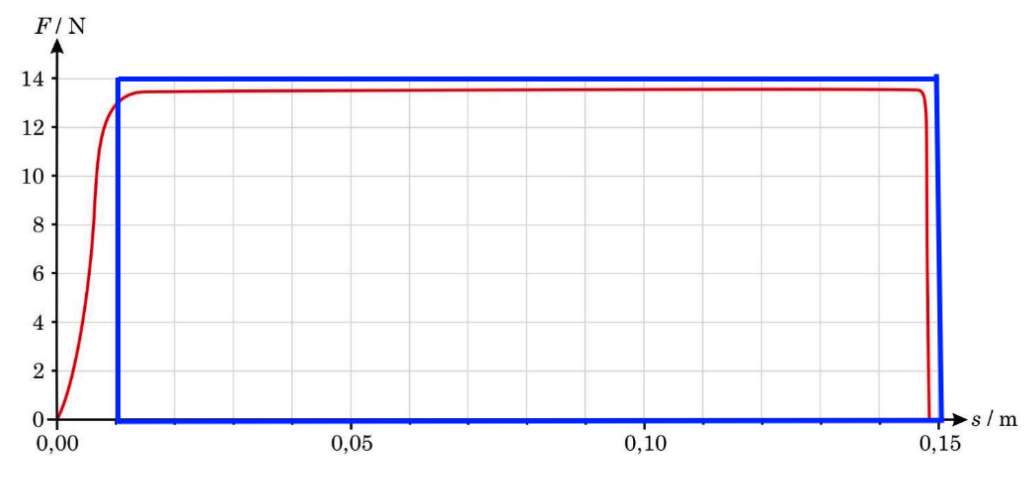
\includegraphics[width=\textwidth]{sF.png}
\end{center}
  \caption{Der tælles cirka 98 tern under $(s,F)$-grafen}
\label{fig:sF}
\end{figure}

\begin{question}{Havvindmølle}{}
  Vingespidserne på en mølle i havvindmølleparken Hywind udfører en jævn cirkelbevægelse medradius 77 m og omløbstid 6,06 s.
\begin{itemize}
  \item[a.] Beregn vingespidsernes fart.
\end{itemize}
Vindmøllerne i Hywind flyder på havet. I roligt vejr flyder en vindmølle stabilt på havet. På grund af bølger stikker vindmøllen på et tidspunkt 1,2 m længere ned under vandoverfladen end i roligt vejr. Møllens opadgående acceleration har på dette tidspunkt størrelsen 0,15 m/s$^2.$
Den del af møllen, som er under havoverfladen, har tværsnitsarealet 154 m$^{2}.$
\begin{itemize}
  \item[b.] Vurder vindmøllens masse
  \item[c.] Vurdér, hvor dybt vindmøllen stikker ned under havoverfladen i roligt vejr.
\end{itemize}
\end{question}
\sol \\
\textbf{a.}
Da vingespidserne netop tilbagelægger omkredsen af cirklen på omløbstiden, så må deres fart være 
\begin{equation*}
\begin{split}
  v&=\frac{2 \cdot \pi \cdot r}{T}\\
  &=\frac{2 \cdot \pi \cdot 77 \;\unit{m} }{6,06 \;\unit{s} }\\
  &\approx 80 \;\unit{m/s}
\end{split}
\end{equation*}
Vingespidsernes fart er altså $80 \;\unit{m/s} $.\\[1ex]
\textbf{b.}
Pga. uafhængighedsprincippe kan vi tillade os blot at kigge på de kræfter, der påvirker vindmøllen i vertikal retning.
Her er det kun opdriften $F_{\text{op} }$ og tyngdekraften $F_t$.
Størrelsen af den resulterende kraft i opadgående retning, må da være 
\[
F _{\text{res} }=F _{\text{op} }-F_t=m \cdot a
\] 
I roligt vejr må der så gælde, at $F _{\text{op} }=F_t$ (for accelerationen er $0$).
Når møllen er mere under vandet, må den positive acceleration opad da skyldes den ekstra opdrift, fordi $F_t$ er konstant. 
Det ekstra volumen af vindmølle under vandet betegnes $V_{\text{stigning} }$.
Altså har vi 
\begin{equation*}
\begin{split}
  F _{\text{res} }= m _{\text{mølle} } \cdot a = \rho_{\text{vand} } \cdot V_{\text{stigning} } \cdot g &\iff m_{\text{mølle} }=\frac{\rho _{\text{vand} }\cdot V _{\text{stigning}} \cdot g}{a}\\
  &\iff m_{\text{mølle} }=\frac{\rho _{\text{vand} }\cdot h _{\text{stigning} } \cdot A \cdot g}{a}
\end{split}
\end{equation*}
hvor $A$ er tværsnitsarealet. 
Vi beregner nu vindmøllens masse.
\begin{equation*}
\begin{split}
  m_{\text{mølle} }&=\frac{\rho _{\text{vand} }\cdot h _{\text{stigning} } \cdot A \cdot g}{a}\\
  &=\frac{1000 \;\unit{kg/m^3} \cdot 1,2 \;\unit{m} \cdot 154 \;\unit{m^2} \cdot 9,82 \;\unit{m/s^2} }{0,15 \;\unit{m/s^2} }\\
  &\approx 12 \cdot 10 ^{6} \;\unit{kg} 
\end{split}
\end{equation*}
Altså er vindmøllens masse $12 \cdot 10^6 \;\unit{kg} $.\\[1ex]
\textbf{c.}
Som sagt gælder der i roligt vejr, at $F _{\text{op} }=F_t$.
Dybden, som vindmøllen stikker ned betegner vi $x$, og vi har da 
\begin{equation*}
\begin{split}
  F _{\text{op} }=F_t &\iff \rho _{\text{vand} } \cdot V _{\text{under} } \cdot g = m_{\text{mølle} } \cdot g\\
  &\iff V _{\text{under} }=\frac{m _{\text{mølle} }}{\rho _{\text{vand} }}\\
  &\iff x \cdot A = \frac{m _{\text{mølle} }}{\rho _{\text{vand} }}\\
  &\iff x=\frac{m _{\text{mølle} }}{\rho _{\text{vand} } \cdot A}
\end{split}
\end{equation*}
Vi beregner nu dybden $x$.
\begin{equation*}
\begin{split}
  x&=\frac{m _{\text{mølle} }}{\rho _{\text{vand} } \cdot A}\\
  &=\frac{12098240 \;\unit{kg} }{1000 \;\unit{kg/m^3} \cdot 154 \;\unit{m^2} }\\
  &\approx 79 \;\unit{m} 
\end{split}
\end{equation*}
Vindmøllen stikker altså $79 \;\unit{m} $ under havoverfladen i roligt vejr. 

\begin{question}{Flexsensorer}{}
En flexsensor har resistansen $23 \;\unit{k \ohm} $, når den ikke er bøjet.
Flexsensoren kan omsætte elektrisk energi med en effekt på 1,0 W.
\begin{itemize}
  \item[a.] Beregn strømstyrken gennem en flexsensor, der ikke er bøjet, når den omsætter elektrisk energi med effekten 1,0 W.
\end{itemize}
Flexsensoren monteres på en finger for at måle, hvor meget fingeren bøjes. 
Flexsensoren er koblet til et elektrisk kredsløb, som vist på diagrammet.
Flexsensoren ændrer resistans, når den bøjes. Herved ændres spændingsfaldet $U_\mathrm{ud}$.
Grafen visen sammenhængen mellem vinklen $v$, som flexsensoren er bøjet, og flexsensorens resistans $R_\mathrm{flex}.$
Ved en bøjning af flexsensoren måles spændingsfaldet $U_\mathrm{ud}$ til 2,1 V.
\begin{itemize}
  \item[b.] Bestem vinklen, flexsensoren er bøjet, når $U_\mathrm{ud}$ er 2,1 V.
\end{itemize}
\end{question}
\sol \\
\textbf{a.}
Effekten, hvormed flexsensoren omsætter elektrisk energi er produktet af spædningsfaldet $U$ over den og strømstyrken $I$ gennem den:
\begin{equation*}
\begin{split}
  P=U \cdot I &\iff P=R \cdot I^2\\
  &\iff I=\sqrt{\frac{P}{R}}
\end{split}
\end{equation*}
da $I$ er positiv. 
Vi kan nu beregne $I$.
\begin{equation*}
\begin{split}
  I&=\sqrt{\frac{P}{R}} \\
  &=\sqrt{\frac{1,0 \;\unit{W} }{23 \cdot 10^3\;\unit{\ohm} }} \\
  &\approx 6,6 \cdot 10 ^{-3} \;\unit{A} 
\end{split}
\end{equation*}
Strømstyrken gennem en ikke-bøjet flexsensor når den omsætter elektrisk energi med effekten $1,0 \;\unit{W} $ er altså $6,6 \cdot 10 ^{-3} \;\unit{A} $. \\[1ex]
\textbf{b.}
På diagrammet ses det, at flexsensoren og resistoren er serieforbundne.
Derudover ses det, at $U_{\text{ud} }$ er spændingsfaldet over resistoren. 
Der gælder altså 
\begin{equation*}
\begin{split}
  U=U _{\text{flex} }+ U _{\text{ud} } \iff U _{\text{flex} }=U-U _{\text{ud} }
\end{split}
\end{equation*}
Vi finder nu et udtryk for strømstyrken gennem resistoren med Ohms lov.
\begin{equation*}
\begin{split}
  U _{\text{ud} }=R _{\text{resistor} } \cdot I\iff I=\frac{U _{\text{ud} }}{R _{\text{resistor} }}
\end{split}
\end{equation*}
Da flexsensoren og resistoren er serieforbundne, så må strømstyrken være konstant og vi kan nu udregne flexsensorens resistans.
\begin{equation*}
\begin{split}
  R _{\text{flex} }&=\frac{U _{\text{flex}}}{I}\\
  &=\frac{U-U _{\text{ud} }}{\frac{U _{\text{ud} }}{R _{\text{resistor} }}}\\
  &=\frac{R _{\text{resistor} }\cdot \left(U-U _{\text{ud} }\right) }{U _{\text{ud} }}\\
  &=\frac{145  \;\unit{k\ohm} \cdot \left(3,0 \;\unit{V} -2,1 \;\unit{V} \right) }{2,1 \;\unit{V} }\\
  &=62,1429 \;\unit{k\ohm} 
\end{split}
\end{equation*}
Vi aflæser på grafen (se \cref{fig:vR}), at vinklen så er $47 \degree $.
Når $U _{\text{ud} }=2,1 \;\unit{V} $ er flexsensoren altså bøjet $47 \degree $. 
\begin{figure}[H]
\begin{center}
  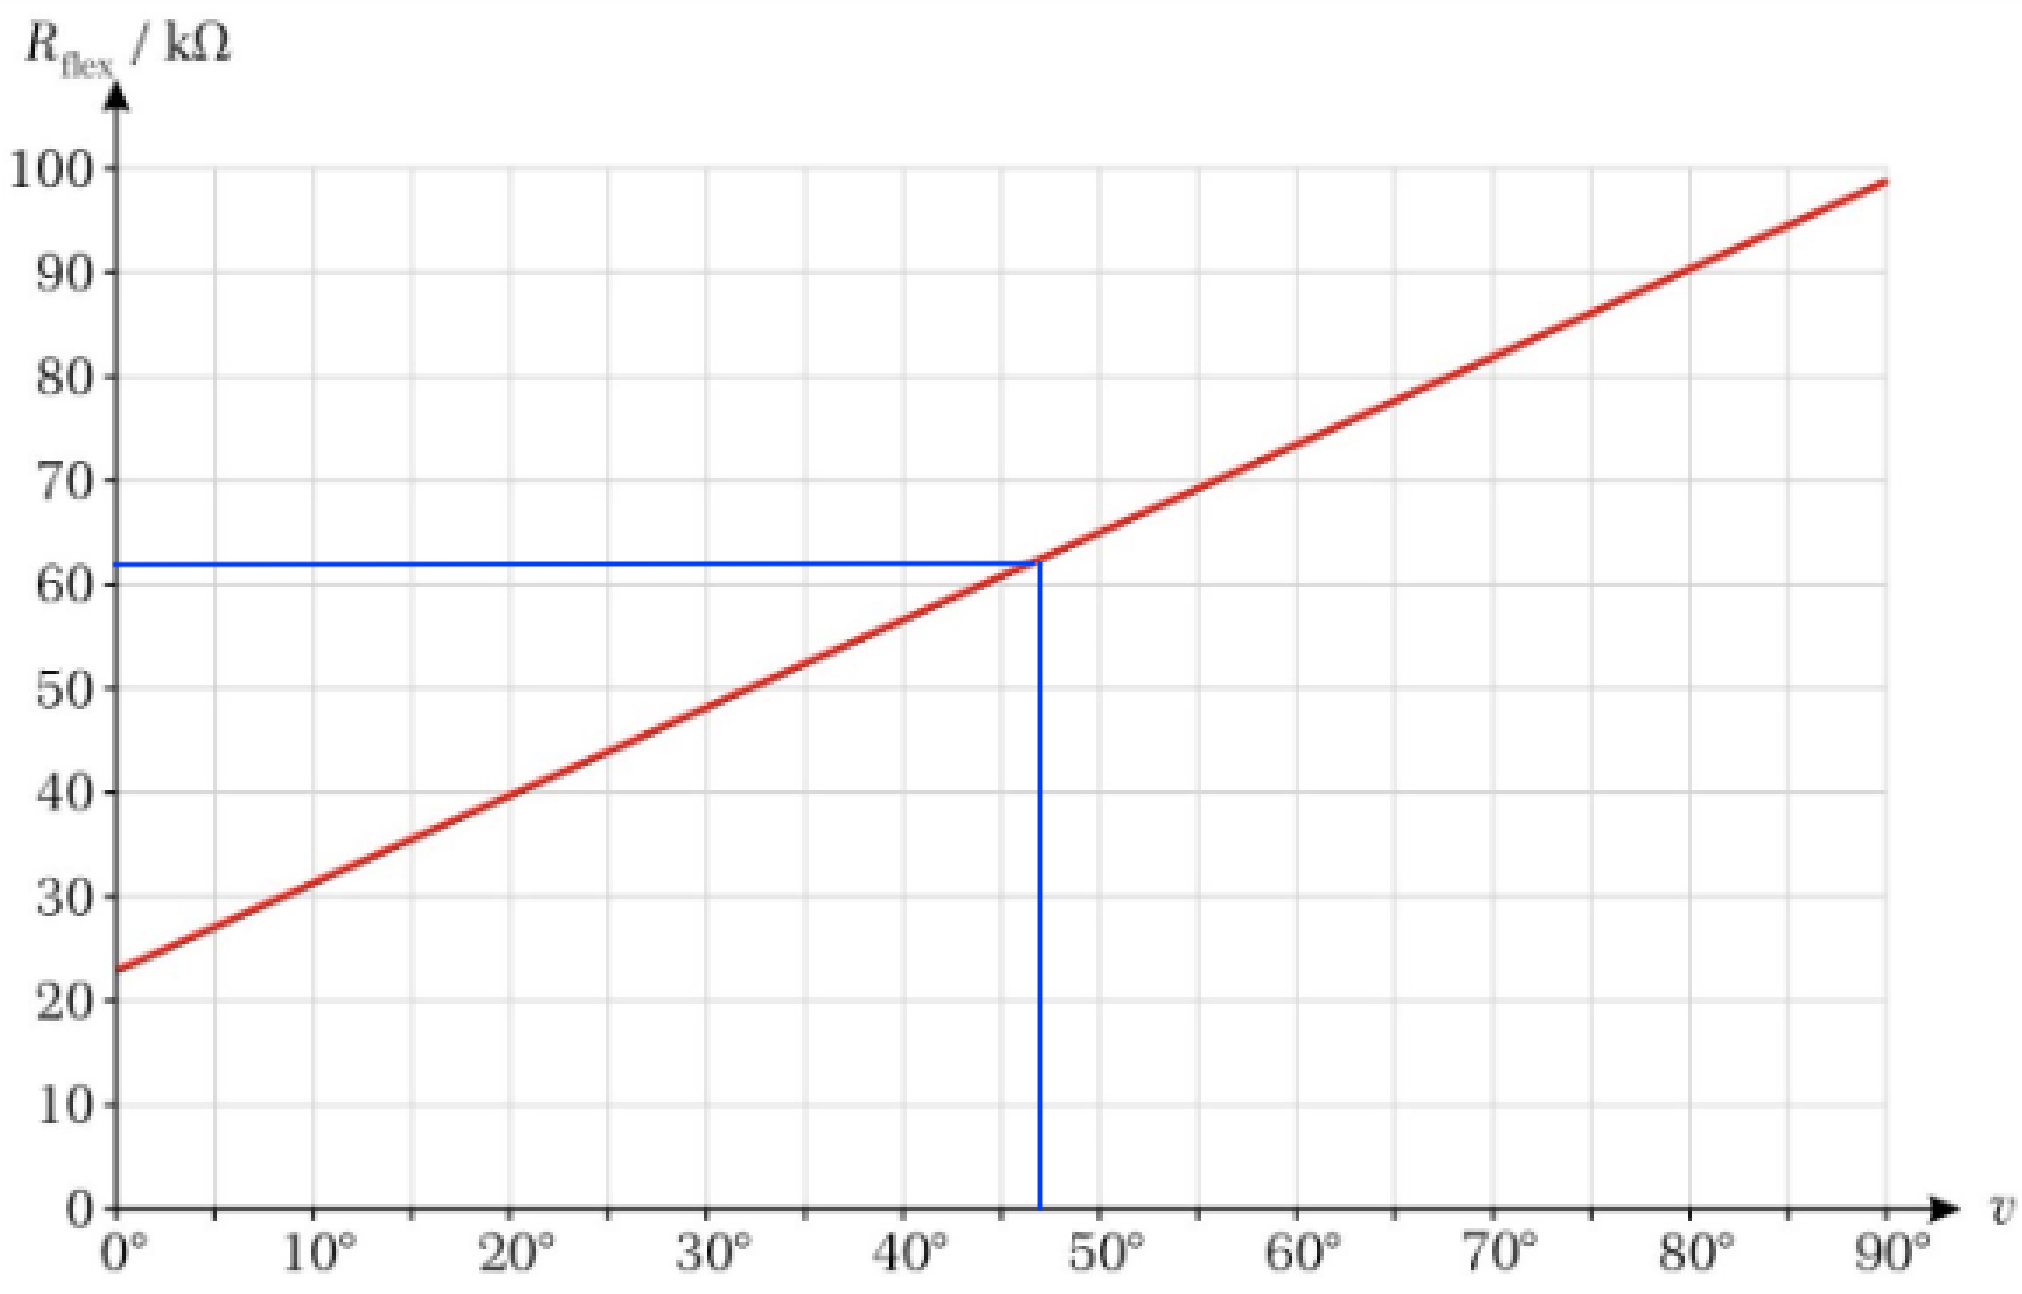
\includegraphics[width=\textwidth]{vR.png}
\end{center}
  \caption{Aflæsning på $(v,R)$-grafen for flexsensoren}
\label{fig:vR}
\end{figure}

\end{document}
